\documentclass[]{report}
\usepackage[hidelinks]{hyperref}
\usepackage{xcolor}
\usepackage{graphicx}
\usepackage{subcaption}
\usepackage{listings}

\lstnewenvironment{sql}
{\lstset{language=SQL,basicstyle=\ttfamily}}
{}

%\usepackage[margin=2cm,footskip=0.25in]{geometry}

\renewcommand{\thefigure}{\arabic{figure}}
\renewcommand{\thetable}{\arabic{table}}
\setlength{\parskip}{6pt}
% Title Page
\title{Vention Data Analysis Report}
\author{Kallil de Araujo Bezerra}


\begin{document}
\maketitle


\tableofcontents

\chapter{Visualization}

The data was received in a \textit{.csv} file, and it contains the following columns:

\begin{itemize}
	\item \textcolor{blue}{\textit{accountid}} - customer account id
	\item \textcolor{blue}{\textit{amount}} - total revenue
	\item \textcolor{blue}{\textit{closedate}} - date in which the deal was closed
	\item \textcolor{blue}{\textit{opportunityid}} - the id of a possible sales lead
	\item \textcolor{blue}{\textit{opportunity\_creation\_date\_\_c}} - date in which the first contact with a customer was made
	\item \textcolor{blue}{\textit{ownerid}} - seller id (the \textit{owner} of the opportunity)
	\item \textcolor{blue}{\textit{primary\_application\_\_c}} - primary application of the product that is being sold
	\item \textcolor{blue}{\textit{stagename}} - in which stage the sale is categorized
	\item \textcolor{blue}{\textit{sales\_team\_\_c}} - to which sales team the opportunity, seller, and customer belongs
\end{itemize}

The description of the columns are based solely on the name of the columns itself. In an ideal environment I would get a more accurate definition of each one by asking the person that sent me the file a description of each column, and proceed with the analysis to avoid mistakes and misinterpretations.

\section{High Level Sales Analysis}

Under the column \textit{stagename} it is possible to see 8 different values, they are:

\begin{itemize}
	\item Closed Lost
	\item Closed Won
	\item Prospect
	\item Project Discovery
	\item Closing Stage
	\item Project Quoted
	\item Design Review
	\item Awaiting Purchase
\end{itemize}

To create a chart that shows which sales had a positive result it was considered the registers that have the value \textit{Closed Won}.

\begin{figure}[htb]
	\centering
	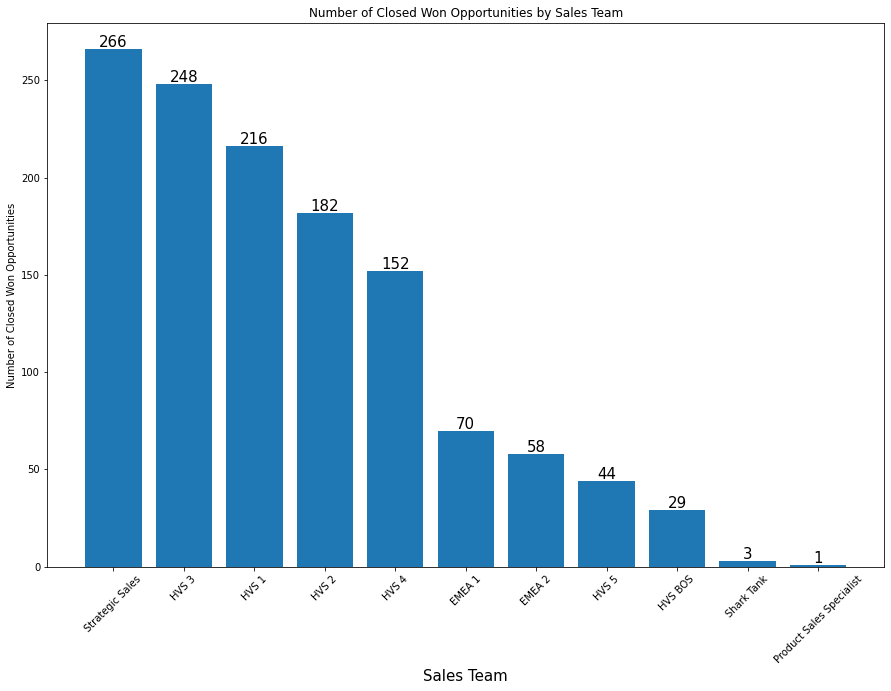
\includegraphics[width=1\textwidth]{fig_01_closed_won}
	\caption{Closed Won versus Sales Team.}
	\label{fig:fig_01}
\end{figure}

As we can see in figure \textcolor{blue}{\ref{fig:fig_01}} the team with most sales is the \textit{Strategic Sales team}, with 266 closed sales won, followed by \textit{HVS 3} and \textit{HVS 1}, with 248 and 216 sales respectively. From now on the analysis will focus on them.

However, it is also important to see the success rate of each team. Even if a team wins many sales, it doesn't mean that it is the most successful because it may be losing many sales too.

To better evaluate this, it was created a \textit{Sales Index}, which can be calculated using the following formula:

\begin{equation}
	Sales\:Index = \frac{\#\:Closed\:Won}{\#\:Closed\:Won + \#\:Closed\:Lost}
\end{equation}

\begin{figure}[htb]
	\centering
	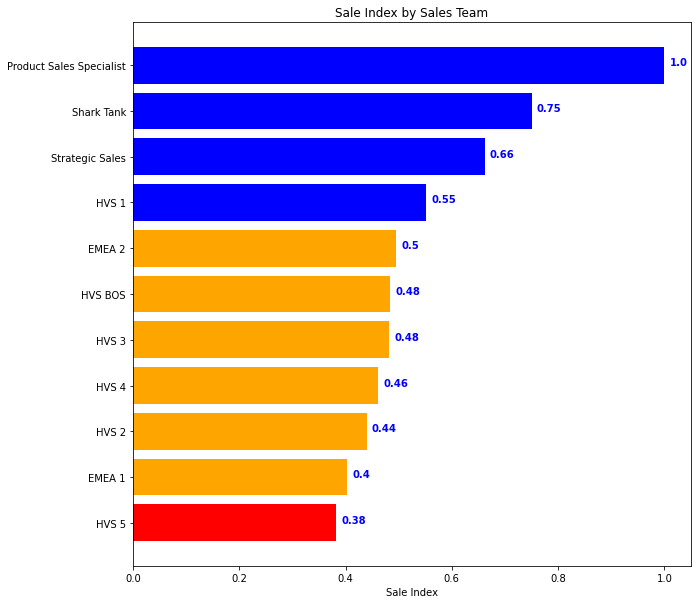
\includegraphics[width=1\textwidth]{fig_02_sales_index}
	\caption{Sales Index.}
	\label{fig:fig_02}
\end{figure}

The color change according to the Sales Index, if it is higher than 0.51 it will be blue, between 0.4 and 0.5 (inclusive) it will be orange, less than 0.4 is red.

From figure \textcolor{blue}{\ref{fig:fig_02}} it is possible to see that some teams have a high value or even a perfect score. However, those teams have a low number of sales, therefore there is a high chance that when they start to grown their sales number, the \textit{Sales Index} will drop. At the same time, the top team is \textit{Strategic Sales}, with a total of 266 sales and a great 66\% Sales Index, or success rate. Knowing which teams are the most successful may help other teams to identify best practices and areas for improvement.

Finally, it is important to show that the teams that are closing more sales are also doing it quick, as can be seen in figure \textcolor{blue}{\ref{fig:fig_02a}}. 

\begin{figure}[htb]
	\centering
	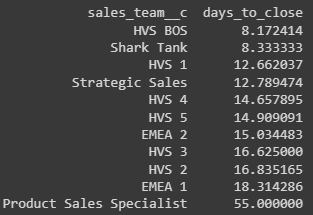
\includegraphics[width=0.55\textwidth]{fig_02_a_days_to_win}
	\caption{Days to close a sale.}
	\label{fig:fig_02a}
\end{figure}

The Strategic Sales and HVS 1 are closing sales in less than two weeks, while the HVS 3 team is spending a little over 16 days.


\subsection{Most sold products by Sales Team}

The next analysis will be more focused on a few teams, the objective is to understand what they sell more and how many days they spend between discovering an opportunity and closing a deal.

The pie charts shown in figures \textcolor{blue}{\ref{fig:fig_03a}}, \textcolor{blue}{\ref{fig:fig_03b}}, and \textcolor{blue}{\ref{fig:fig_03c}} present which products are more relevant to each of the top 3 teams (Strategic Sales, HVS 1, and HVS 3). The \textit{Other Products} are the ones that are not in the top 5, however, it is important to keep them in the visualization so we can see their impact in each team.

From the pie charts it is possible to see that those teams are specialized in different areas. Strategic Sales is strong with Robot Pedestals and Bases, HVS 1 is divided between Safety Enclosures and Workstations, and HVS 3 is experienced with Robot Range Extender. However, all three have at least 10\% of sales related to Workstations, therefore, this area is important for all teams.

\begin{figure}[htb]
	\centering
	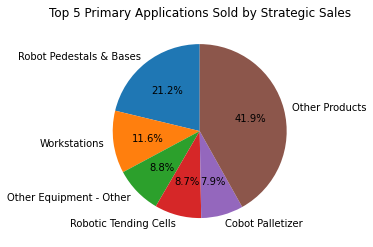
\includegraphics[width=0.85\textwidth]{fig_03_strategic_sales}
	\caption{Products sold by Strategic Sales}
	\label{fig:fig_03a}
\end{figure}

\begin{figure}[htb]
	\centering
	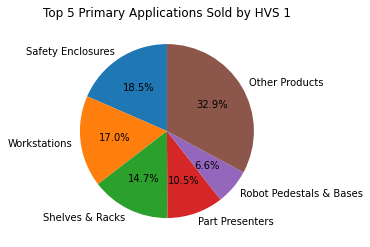
\includegraphics[width=0.85\textwidth]{fig_03_hvs_1}
	\caption{Products sold by HVS 1}
	\label{fig:fig_03b}
\end{figure}

\begin{figure}[!t]
	\centering
	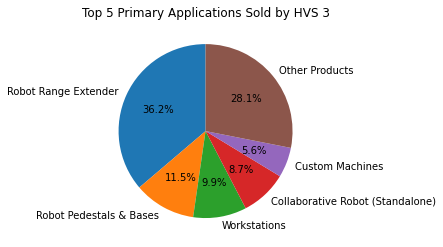
\includegraphics[width=1\textwidth]{fig_03_hvs_3}
	\caption{Products sold by HVS 3}
	\label{fig:fig_03c}
\end{figure}


\clearpage
\section{Strategic Sales Team}

In this section the Strategic Sales Team will be better analyzed, so we can understand who are the owners of the opportunities and how many sales they did. 

\begin{figure}[htb]
	\centering
	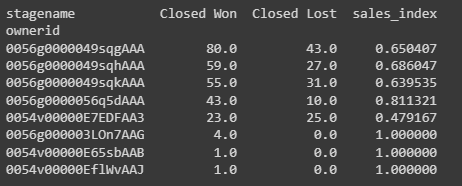
\includegraphics[width=0.70\textwidth]{fig_04_sellers}
	\caption{Sellers and their indexes}
	\label{fig:fig_04}
\end{figure}

In figure \ref{fig:fig_04} it is shown the total Closed Won and Closed Lost sales by each of the sellers in the Strategic Sales team, most of them present a good Sales Index. However the seller \textit{0054v00000E7EDFAA3} seems to lose more customers than win new ones. Therefore, it is important to further investigate why this is happening and find a solution.

A possible cause for the low performance of the seller \textit{0054v00000E7EDFAA3} might be a overwhelming number of customers. Therefore lets analyze the how many customers each of the sellers have. The result can be seen in figure \ref{fig:fig_05}.

\begin{figure}[htb]
	\centering
	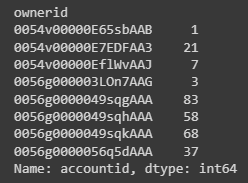
\includegraphics[width=0.50\textwidth]{fig_05_customer_and_sellers}
	\caption{Amount of clients by sellers}
	\label{fig:fig_05}
\end{figure}

As we can see, the number of costumers that the seller \textit{0054v00000E7EDFAA3} is managing is not high, so it may need further investigation.

\section{HVS 1}

Now we will execute the same analysis with the team HSV 1. Which gives the results from figure \textcolor{blue}{\ref{fig:fig_06}}.

\begin{figure}[htb]
	\centering
	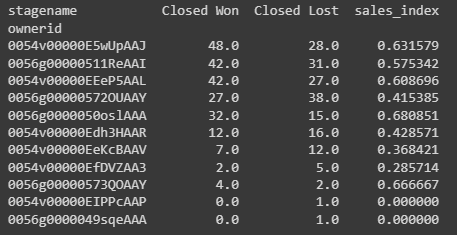
\includegraphics[width=0.70\textwidth]{fig_06_sellers_hs1}
	\caption{Sellers and their indexes - HVS 1}
	\label{fig:fig_06}
\end{figure}

As the analysis show, there are many seller with low performance indexes. Despite being one of the top teams in the company, HSV 1 has a high number of low performing sellers. Therefore, further investigation is needed.

\begin{figure}[htb]
	\centering
	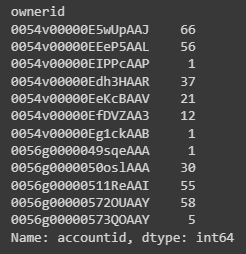
\includegraphics[width=0.50\textwidth]{fig_06_customers_and_sellers_hs1}
	\caption{Amount of clients by sellers - HVS 1}
	\label{fig:fig_07}
\end{figure}

The amount of customers that each seller is managing in HVS 1 is higher, therefore it's possible that they are overloaded and may need help.

%\section{HVS 3}

\chapter{SQL query}

This chapter will be dedicated to discuss the implementation and query to solve the second task.

\section{Database creation}

To complete this task it was necessary to understand how the tables were related, so a version of what is presented in the task was implemented. The Entity Relation Diagram (ERD) can be seen in figure \textcolor{blue}{\ref{fig:fig_08}}.

This diagram was created using the \textit{PGAdmin} tool \textit{ERD for Database}. Moreover, fake data was used to populate the database. Users and products are related to the \textit{Star Wars} universe, and as this database was created only for test purposes, there isn't a high amount of data on it. Some users have a email that ends in \textit{@vention.cc} to add a condition that should be met, according to the Technical Test.

At first the implementation tried to follow a star schema, but the way that the data is related is closer to a snowflake schema. Therefore, a new data model would be needed to use a star schema and the end result would be very different from what was shown.

The query can be seen in table \textcolor{blue}{\ref{tbl:sql_query}} in addition to that, images \textcolor{blue}{\ref{fig:fig_08}} and \textcolor{blue}{\ref{fig:fig_09}}

\begin{table}[h]
	\centering
	\begin{tabular}{l}
		\hline
		\textbf{SQL Query} \\
		\hline
		\begin{minipage}[t]{0.9\textwidth}
			\begin{verbatim}
				SELECT date_trunc('month', o.created_at) AS order_month,
				 COUNT(DISTINCT o.id) AS count_orders,
				 SUM(CASE
				  WHEN opli.partner_id IS NULL THEN oli.item_price * oli.quantity
				  ELSE opli.item_price * pf.contract_rate * opli.quantity
				 END) AS total_gross_sales,
				 SUM(CASE
				  WHEN opli.partner_id IS NULL THEN oli.item_cost * oli.quantity
				  ELSE opli.item_price * opli.quantity
				 END) AS total_net_sales,
				 array_agg(o.id) AS list_order
				FROM orders o
				JOIN order_line_items oli ON o.id = oli.order_id
				LEFT JOIN order_partner_line_items opli 
				  ON o.id = opli.order_id AND oli.part_number = opli.part_number
				LEFT JOIN partner_feature pf 
				  ON opli.partner_id = pf.id
				JOIN users u ON o.user_id = u.id
				WHERE u.email NOT LIKE '%@vention.cc'
				AND o.created_at >= '2021-01-01'
				GROUP BY order_month
				ORDER BY order_month;
			\end{verbatim}
		\end{minipage} \\
		\hline
	\end{tabular}
	\caption{Final Query - Exercise 02}
	\label{tbl:sql_query}
\end{table}


\begin{figure}[htb]
	\centering
	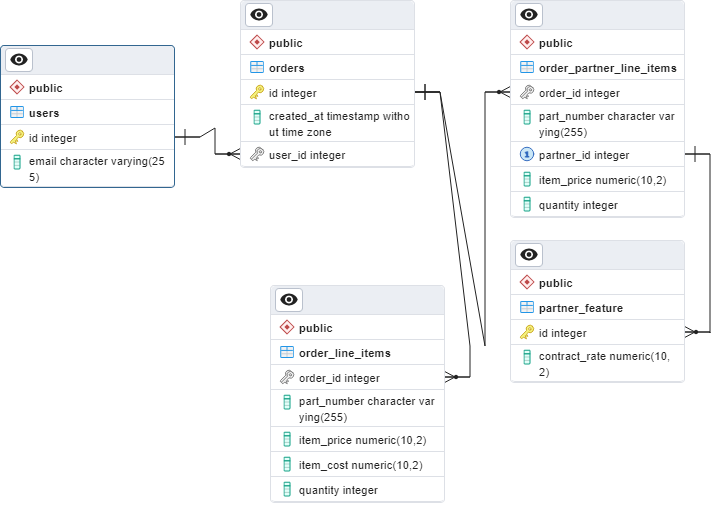
\includegraphics[width=1.1\textwidth]{01_data_modeling_resize}
	\caption{ERD of the implemented database}
	\label{fig:fig_08}
\end{figure}

\begin{figure}[htb]
	\centering
	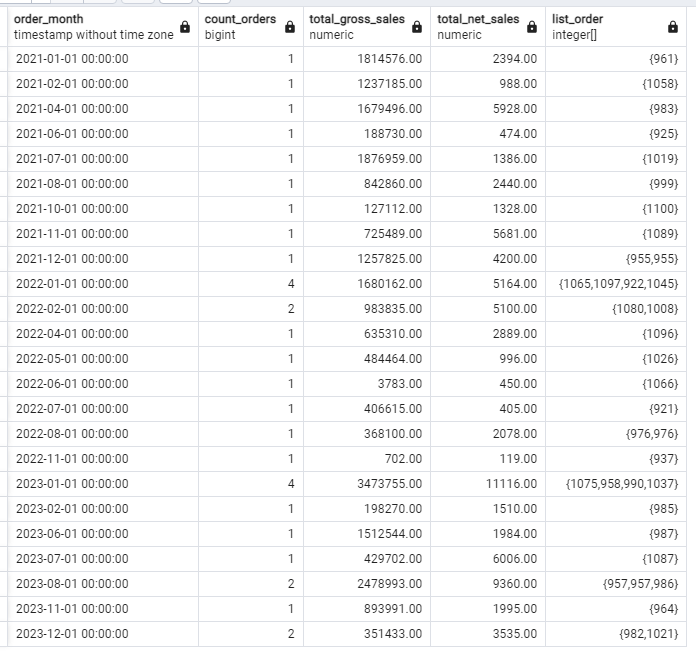
\includegraphics[width=1.3\textwidth]{02_result_01}
	\caption{Query result}
	\label{fig:fig_09}
\end{figure}



\chapter{Technical details}

All of the data, code, and images that were used here can be found at \href[]{https://github.com/Kallil12/Step_3}{\textcolor{blue}{Kallil's Github}}.


\end{document}          
